\chapter{Diseño de la interfaz de usuario}

Una vez hemos definido cuáles son nuestros objetivos, analizado el estado del arte y establecido unas pautas para el desarrollo, vamos a comenzar con el diseño de la parte visual. Esto es, a su vez, un proceso que requiere de distintas definiciones, de manera que al término de este capítulo, no sólo tengamos el diseño de las interfaces de usuario, sino que también comprendamos por qué se han diseñado así y la intención de cada elemento que disponemos en pantalla.

\section{Matriz de tareas de usuario}

Un buen comienzo sería el de definir los roles de usuario en nuestra nueva aplicación. Hemos hablado ya en el capítulo anterior sobre la figura del \gls{gestortwinX} y la del \gls{administradortwinX}. Incluyamos entonces también las de \gls{Tutor}, estudiante y, de forma excepcional, la de coordinador(a) externo/a. Sobre esta última, recordemos que no tenía ningún tipo de interacción en TWINS y que hasta entonces, los usuarios de la plataforma habían establecido intercambios de información por correo electrónico con los coordinadores de otras facultades, que es el método estándar de realizar las \glspl{Nominacion}. Sin embargo, aunque no para sus primeras versiones, se espera que twinX brinde la capacidad de hacer estas nominaciones a través de una interfaz gráfica, de una forma mucho más sencilla y segura que con el envío de un texto libre, donde puede haber errores y/o malas prácticas, dado el amplio uso que se puede hacer de la herramienta.

Es precisamente por la necesidad de dejar claras las acciones a llevar a cabo por cada usuario del sistema por la que elaborar una \textbf{matriz de tareas de usuario}. Esta herramienta nos permite establecer cuál es la frecuencia de uso de una característica de nuestra aplicación por un grupo de usuarios en concreto y cuál es la prioridad que debemos darle a la implementación de la misma. De esta forma, nos será más fácil diferenciar aquellas acciones que tan solo se lleven a cabo unas pocas veces al mes (o cada varios meses) y cuales, por el contrario, son ejecutadas casi a diario, de modo que se priorice su integración y su optimización. Sobre estas últimas, cabe decir que el potenciarlas no solo se procurará hacer en términos de procesamiento interno del código, sino también en cuanto a su facilidad de utilización por parte del usuario. Es decir, tendremos que crear más accesos directos o simplificar lo máximo posible el curso de tareas a llevar a cabo para realizar estas acciones y obtener los resultados deseados. En adición a todo esto, podremos observar cuáles son los usuarios que menos usarán la plataforma, de modo que se reste prioridad a la implementación de sus interacciones, en beneficio de las que llevan a cabo los usuarios que, por el contrario, monopolizan el uso de la aplicación \cite{matrizTareas}.

Para simplificar la matriz (tabla \ref{tab:matrizTareas}) y hacerla visualmente más sencilla de entender, vamos a asignar una serie de letras que correspondan a un nivel de utilización en concreto. Elegiremos la «A» para una frecuencia de uso alta, «M» para un uso medio y «B» para una baja frecuencia. A estas indicaciones añadiremos unas puntuaciones que nos permitirán determinar con mayor facilidad cuáles son las tareas de mayor importancia y cuáles son menos urgentes de implementar, al igual que los usuarios que desempeñarán un papel más o menos crítico en la aplicación. Respectivamente serán 3, 2 y 1 punto, de modo que las prioridades más altas recibirán una mayor puntuación y viceversa.

\begin{table}[h]
	\begin{center}
		\begin{adjustbox}{width=1\textwidth}
			\begin{tabular}{ | >{\centering\arraybackslash}p{0.375\linewidth} | c | c | c | c | c | c | } 
				\hline
				\textbf{Usuarios / Tareas} & \textbf{Administrador} & \textbf{Gestor} & \textbf{Tutor} & \textbf{Estudiante} & \textbf{Coordinador externo} & \textbf{Puntuación} \\
				\hline
				Acceder a twinX & M & A & B & B & B & \cellcolor{red!25}8 \\
				\hline
				Ver expedientes de un usuario & A & A & & & & \cellcolor{red!25}6 \\
				\hline
				Cambiar de fase un expediente & A & A & & & & \cellcolor{red!25}6 \\ 
				\hline
				Consultar la información de un convenio & A & A & & & & \cellcolor{red!25}6 \\ 
				\hline
				Modificar los datos de un estudiante & M & M & & B & & \cellcolor{red!25}5 \\
				\hline
				Introducir un nuevo convenio & B & M & & & & 3 \\
				\hline
				Realizar el acuerdo de estudios & & & & B & & 1 \\
				\hline
				Revisar propuesta de acuerdo de estudios & & B & M & & & 3 \\
				\hline
				Consultar los expediente pendientes de procesamiento & M & A & & & & 5 \\
				
				\hline
				Expresar consentimiento de cesión de datos & & & & B & & 1 \\
				\hline
				Añadir un nuevo tipo de expediente y/o fase de expediente & B & & &  & & 1 \\
				\hline
				Marcar un expediente como favorito & B & M & & & & 3 \\
				\hline	
				\textbf{Puntuación del grupo de usuarios} & \cellcolor{red!25}18 & \cellcolor{red!25}22 & 3 & 4 & 1 &  \\
				\hline
		\end{tabular}
	\end{adjustbox}
		\caption{Matriz de tareas de usuario}
		\label{tab:matrizTareas}
	\end{center}
\end{table}

Tras la atenta observación de la matriz, podemos afirmar que las acciones que mayor uso van a tener por los usuarios de twinX serían las ya existentes en TWINS, como es lógico, y que por supuesto, los grupos de usuarios con mayor necesidad de uso de la aplicación son los gestores y administradores. Sobre éstos últimos, cabe señalar que son una especie de gestores con más permisos de lo normal, de modo que pueden modificar la información que clasifica la situación de los estudiantes como son, por ejemplo, las fases de los expedientes. Solo los administradores podrían hacerlo, ya que los gestores no tienen por qué tener acceso a dichas modificaciones; simplemente necesitan trabajar con las ya registradas y, en caso de necesitar más entradas o la modificación de otras existentes, tendrían que solicitarlo a los administradores.

Con esta matriz, además, justificamos que el contenido de la primera versión de twinX (descrito en la sección~\ref{subsec:propuesta}), es suficiente para cubrir la mayoría de las necesidades esenciales del trabajo de un secretario de la ORI-FyL, lo que es uno de los objetivos principales de este proyecto, aunque sea tan solo un comienzo a lo que finalmente llegaría a ser twinX.

\section{Mapa web (sitemap)}

Cuando un usuario llega a un sitio web por primera vez, incluso si es experimentado, no sabe qué hacer o dónde hacer clic. Lo normal es que esta duda no perdure por más de 15 segundos en la cabeza, aunque podría ser así si el sitio web en cuestión no tiene una estructura bien definida.

Para aclarar la estructura de un portal web, se puede hacer uso de los \textit{sitemaps}. Es un esquema visual que permite mostrar la arquitectura de la información en el sitio, y qué secciones están enlazadas y/o relacionadas.

Aparte de definir, este tipo de diagramas nos permite comprender mejor nuestros objetivos, si vamos bien encaminados y tenemos una idea que es válida también para los usuarios finales del producto y si por algún motivo hemos de eliminar páginas innecesarias o que puedan ser redundantes.

Para su confección, es necesario disponer la página de inicio y las secciones que parten de ahí y que llevan a otros sitios, a modo de árbol. Una buena estrategia es la de tratar de minimizar el número de pasos que hay que dar para llegar a encontrar la información deseada desde el comienzo del diagrama. Esto es lo que conocemos como \textbf{la regla de los 3 clics}; aunque no oficial, es sin duda una apuesta segura para la simplicidad, facilitando que los usuarios menos experimentados puedan usar el sitio sin tener que dedicar mucho tiempo a ello, en cuyo caso podrían abandonar y buscar otra alternativa \cite{sitemap}.

\begin{figure}
	\centering
	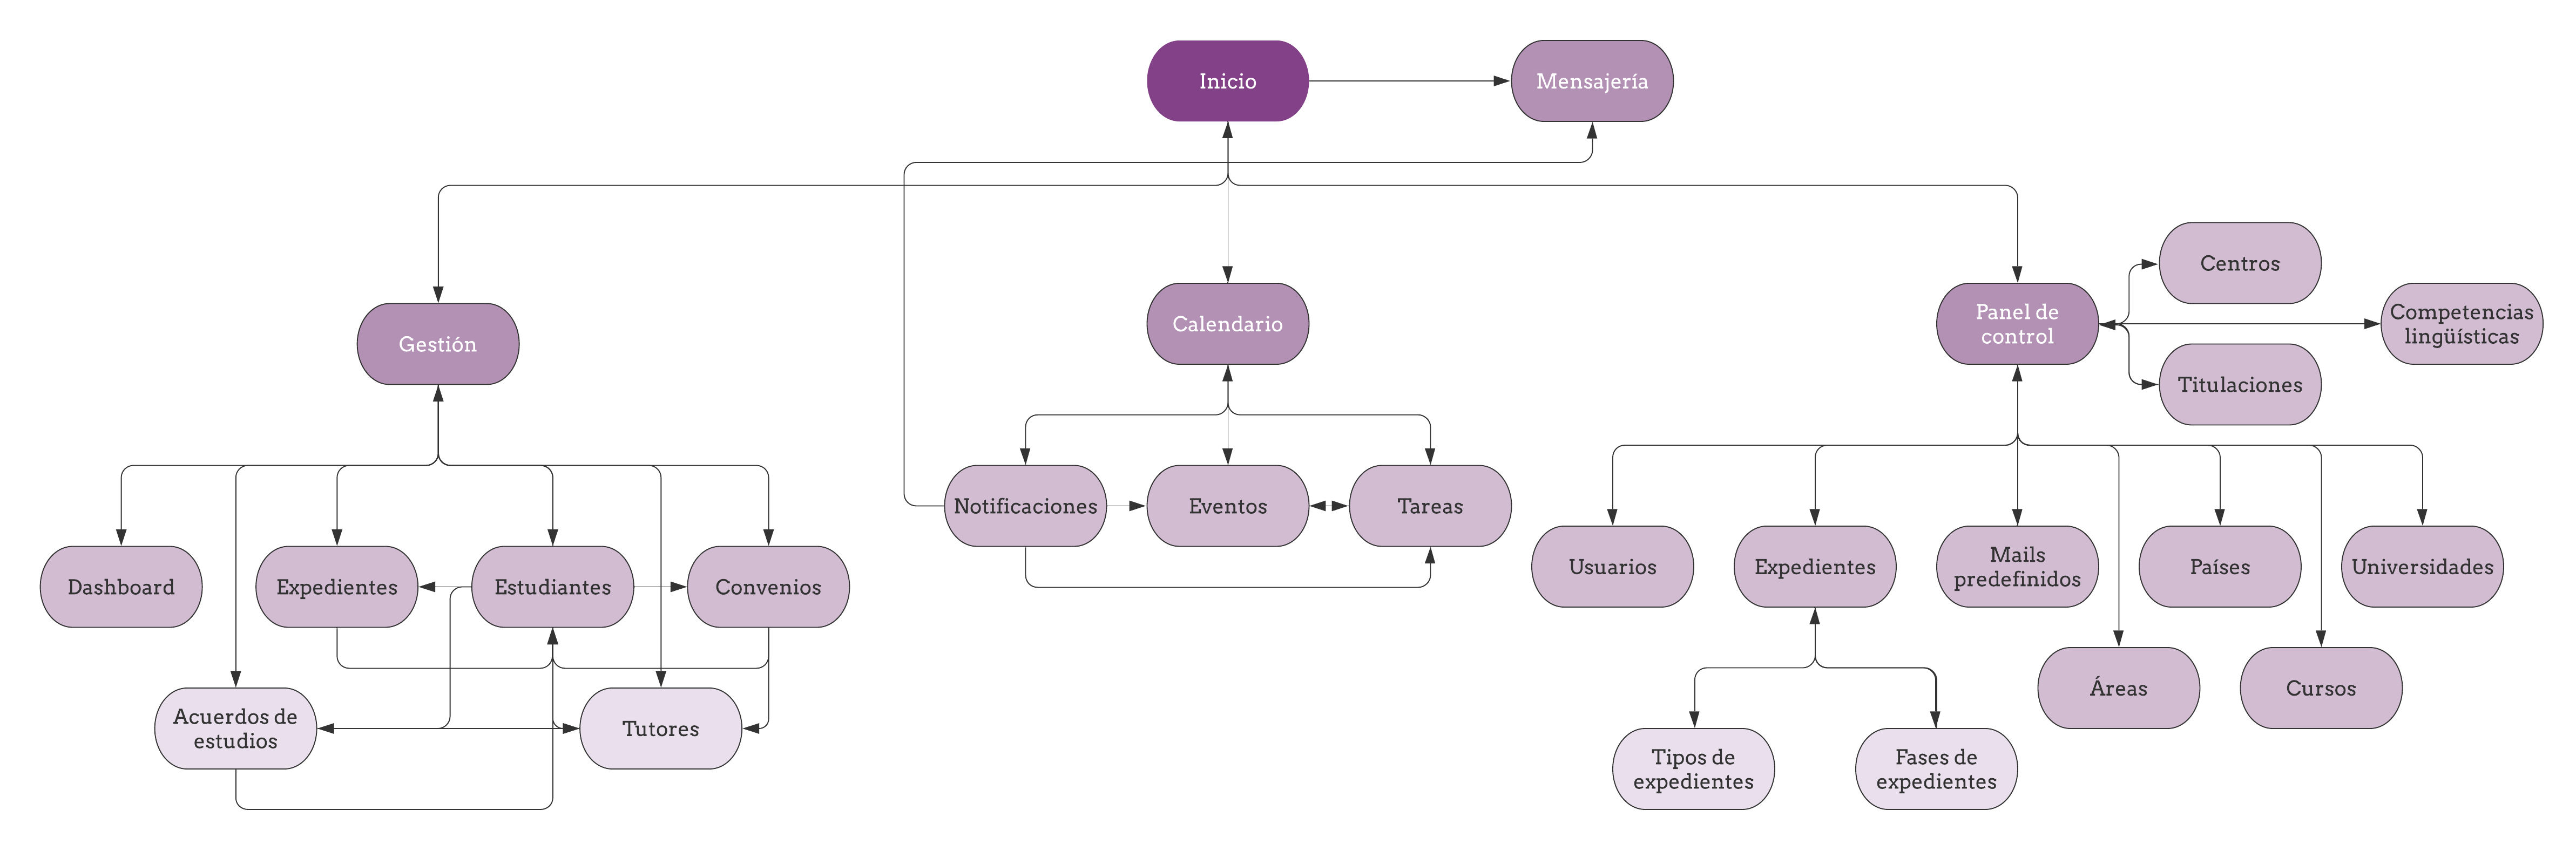
\includegraphics[width=\textwidth]{img/sitemap}
	\caption{Sitemap de twinX}
	\label{fig:sitemap}
\end{figure}

En la figura \ref{fig:sitemap} exponemos el \textit{sitemap} de twinX, diferenciando claramente sus tres secciones principales: gestión, calendario y panel de control. En la parte de gestión, destaca la cantidad de posibilidades de navegabilidad existentes, dado que por ejemplo, al buscar un expediente en su menú, podríamos acceder al perfil de un estudiante o viceversa. Lo mismo pasa con los convenios y los acuerdos de estudios: todos estos accesos directos se ponen para facilitar el trabajo del usuario y mejorar su experiencia, usando los menús ya creados y evitando la redundancia de los mismos.


\section{Iconografía (labelling)}

Resultaría muy extraño navegar hoy en día por una web que no tuviera un icono ofreciendo alguna indicación. Quizás, al pensar en la palabra «icono» nos vengan a la cabeza expresiones faciales que utilizamos a diario para comunicarnos (los famosos emoticonos), pero lejos de adornar, estos símbolos gráficos nos facilitan mucho la navegación por internet con indicaciones visuales que nos hacen ahorrar tiempo para encontrar un menú desplegable, el botón para iniciar sesión o simplemente la salida.

Como no podía ser de otra forma, nuestro portal no es una excepción y también incluye iconos para mejorar la experiencia de navegación. En la tabla \ref{tab:iconografia} presentamos los iconos existentes en twinX.

\begin{table}[h]
	\begin{center}
		\begin{adjustbox}{width=1\textwidth}
			\begin{tabular}{ | >{\centering\arraybackslash}p{0.375\linewidth} | >{\centering\arraybackslash}p{0.375\linewidth} | c | c | } 
				\hline
				\textbf{Etiqueta} & \textbf{Descripción} & \textbf{Icono} & \textbf{Etiqueta (inglés)} \\
				\hline
				Sobre & Consultar el menú de envío de emails de un expediente concreto en el panel de control & \pbox{4cm}{\bigskip \huge\faEnvelope}  & \textit{Envelope} \\ 
				\hline
				Ojo & Ver el detalle de los datos almacenados para una determinada entrada en una lista & \pbox{4cm}{\bigskip \huge\faEye}  & \textit{Eye} \\ 
				\hline
				Lápiz & Editar la información de una entrada concreta en una lista & \pbox{4cm}{\bigskip \huge\faPencil}  & \textit{Pencil} \\ 
				\hline
				Papelera & Eliminar una entrada de una lista & \pbox{4cm}{\bigskip \huge\faTrash}  & \textit{Trash} \\ 
				\hline
				Flecha de desplegable (\textit{dropdown}) hacia abajo & Indicador de la dirección del despliegue del menú \textit{dropdown} & \pbox{4cm}{\bigskip \huge\faCaretDown}  & \textit{Caret down} \\ 
				\hline
			
			\end{tabular}
		\end{adjustbox}
	\caption{Iconos de twinX}
	\label{tab:iconografia}
	\end{center}
\end{table}

\section{Guía de estilo}

En \hyperref[reunion3]{reunión de presentación de TWINS}, Miguel Ángel comentó los significados del logo de TWINS (figura \ref{fig:logotwins}) y el por qué de los dos colores. Representan la unión de los estudiantes OUT (en color rojo) con los estudiantes IN (en azul), que se engarza en un corazón morado con motivo de la unión de dos universidades. Hemos querido mantener este concepto para la construcción de twinX, y la apuesta por una tipografía más vistosa como es Quicksand \cite{quicksand}. Para la coloración, hemos escogido los dos colores emblemáticos de la aplicación para mezclarlos un morado que va a ser el protagonista de los detalles en toda la web. Como resultado, se tiene el logo de la figura \ref{fig:logotwinX}, el utilizado en la cabecera de la web.

\begin{figure}
	\centering
	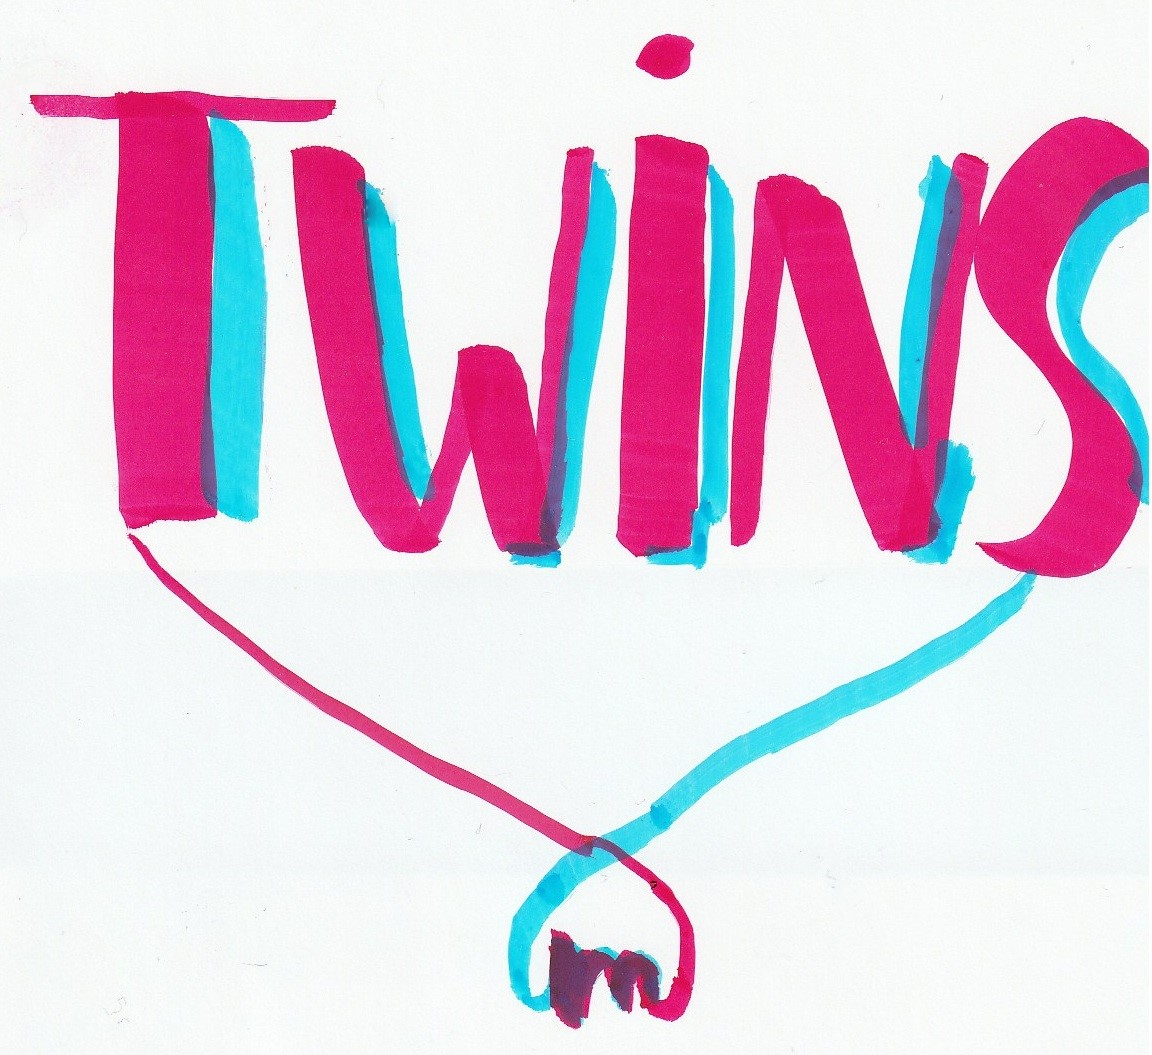
\includegraphics[width=0.7\textwidth, height=0.4\textheight]{img/logotwins}
	\caption{Logo de TWINS}
	\label{fig:logotwins}
\end{figure}

\begin{figure}
	\centering
	
\includegraphics[width=\textwidth]{img/logo}
	\caption{Logo de twinX}
	\label{fig:logotwinX}
\end{figure}

Sobre los colores, hemos usado la herramienta \textbf{Color Tool} de \textit{Material Design} para establecer el esquema de colores (figura \ref{fig:esquemacolores}). Hemos usado mayormente el tono normal (\#ba68c8) y el oscuro (\#883997) para twinX, siendo éste último el empleado en las partes seleccionadas o cabeceras de tablas y el primero, para todo lo demás en cuanto a detalles (hiperenlaces, en su mayoría).

La fuente utilizada ha sido \textbf{Segoe UI} \cite{segoeui}, por tener buena concordancia con la escogida para el logo, su buena legibilidad y su simplicidad (figura \ref{fig:segoeui}).

\begin{figure}
	\centering
	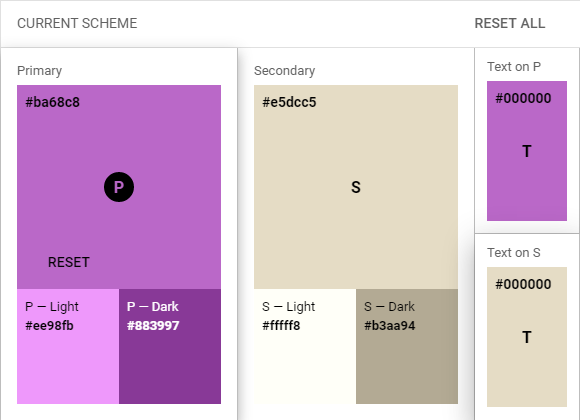
\includegraphics{img/esquema_colores}
	\caption{Esquema de colores de twinX}
	\label{fig:esquemacolores}
\end{figure}

\begin{figure}
	\centering
	
\includegraphics{img/segoeui}
	\caption{Tipografía Segoe UI}
	\label{fig:segoeui}
\end{figure}


\section{Bocetos wireframe}

Con gran parte de los elementos necesarios definidos para poder crear twinX, necesitamos tener una idea clara de interfaz de usuario en mente antes de poder comenzar a integrarla. Pensemos lo fácil que es corregir errores de diseño tan solo arrastrando elementos y disponiéndolos en el boceto. Gracias a eso, podemos ahorrar mucho tiempo a la hora de programar según la guía que suponen los \textit{wireframes}.

\subsection{Wireframes del módulo de gestión}

Para el módulo de gestión, tenemos los siguientes bocetos:

\begin{itemize}
	\item \textbf{\hyperref[fig:dashboardWF]{Dashboard}:} una sección nueva que proponemos para twinX, donde se puede ver de un vistazo la información más importante para el usuario. Recordemos que en TWINS, al principio se disparaban una serie de vistas de calendario, avisos y tareas, etc. Todo ello obligaba al usuario a cerrar ventanas posiblemente indeseadas. Con esta nueva aproximación, el objetivo es aumentar la efectividad en el trabajo, pudiendo redirigirse a múltiples instancias del portal web desde un único lugar.
	\item \textbf{\hyperref[fig:convenios_listaWF]{Lista de convenios}:} manteniendo la información de mayor utilidad para el usuario, como el número de estudiantes salientes y/o entrantes que hay en destino del total de estudiantes que han sido nominados para ese convenio.
	\item \textbf{\hyperref[fig:vista_conv_basica_contWF]{Vista de convenios básica contraída}:} en TWINS había dos posibilidades para visualizar un convenio: estaba la vista básica, con la información de mayor relevancia para las consultas diarias; y la avanzada, que mostraba todos los detalles que se tenían sobre un convenio en concreto. Sin embargo, estaban en vistas distintas. En twinX, proponemos un único menú de convenio con un botón para cambiar entre la vista básica y la vista avanzada.
	\item \textbf{\hyperref[fig:vista_conv_avanzada_contWF]{Vista de convenios avanzada contraída}:} con todas las secciones contenedoras de los datos que alberga un convenio en su totalidad.
	\item \textbf{\hyperref[fig:vista_conv_extendidaWF]{Vista de convenios extendida}:} para ver los detalles de una o varias secciones del convenio en concreto.
	\item \textbf{\hyperref[fig:expedientes_listaWF]{Lista de expedientes}:} se incluyen accesos directos a acciones rápidas que facilitan el trabajo de los gestores, como se venía haciendo en TWINS.
	\item \textbf{\hyperref[fig:estudiantes_listaWF]{Lista de estudiantes}:} de nuevo, con accesos directos para agilizar las operaciones.
	\item \textbf{\hyperref[fig:busquedaWF]{Búsqueda con desplegable}:} con la posibilidad de aplicación de distintos filtros para obtener unos mejores resultados. Éstos también tienen accesos directos que agilizan el trabajo. Por ejemplo, si se quisieran consultar los expedientes de un usuario, se podría ir directamente a ellos, sin tener que recuperar previamente la información del usuario en cuestión por completo.
	\item \textbf{\hyperref[fig:expediente_detalleWF]{Vista de expediente}:} con información de relevancia para el gestor sobre el estudiante y una lista de las fases por las que el expediente ha pasado hasta la más actual. Se permite adjuntar documentación a cada fase y procesar un cambio de fase desde esa misma vista, para simplificar el desdoble en menús. También se incluye la posibilidad de crear una nueva fase.
	\item \textbf{\hyperref[fig:cambio_faseWF]{Diálogo modal de cambio de fase}:} avisa al usuario de las acciones que se van a desarrollar tras la confirmación del procesamiento de la fase, que será principalmente el envío automatizado de mails predefinidos.
	\item \textbf{\hyperref[fig:estudiante_detalleWF]{Vista de estudiante}:} donde se dispone toda la información acerca de un estudiante.
\end{itemize}

\begin{figure}
	\centering
	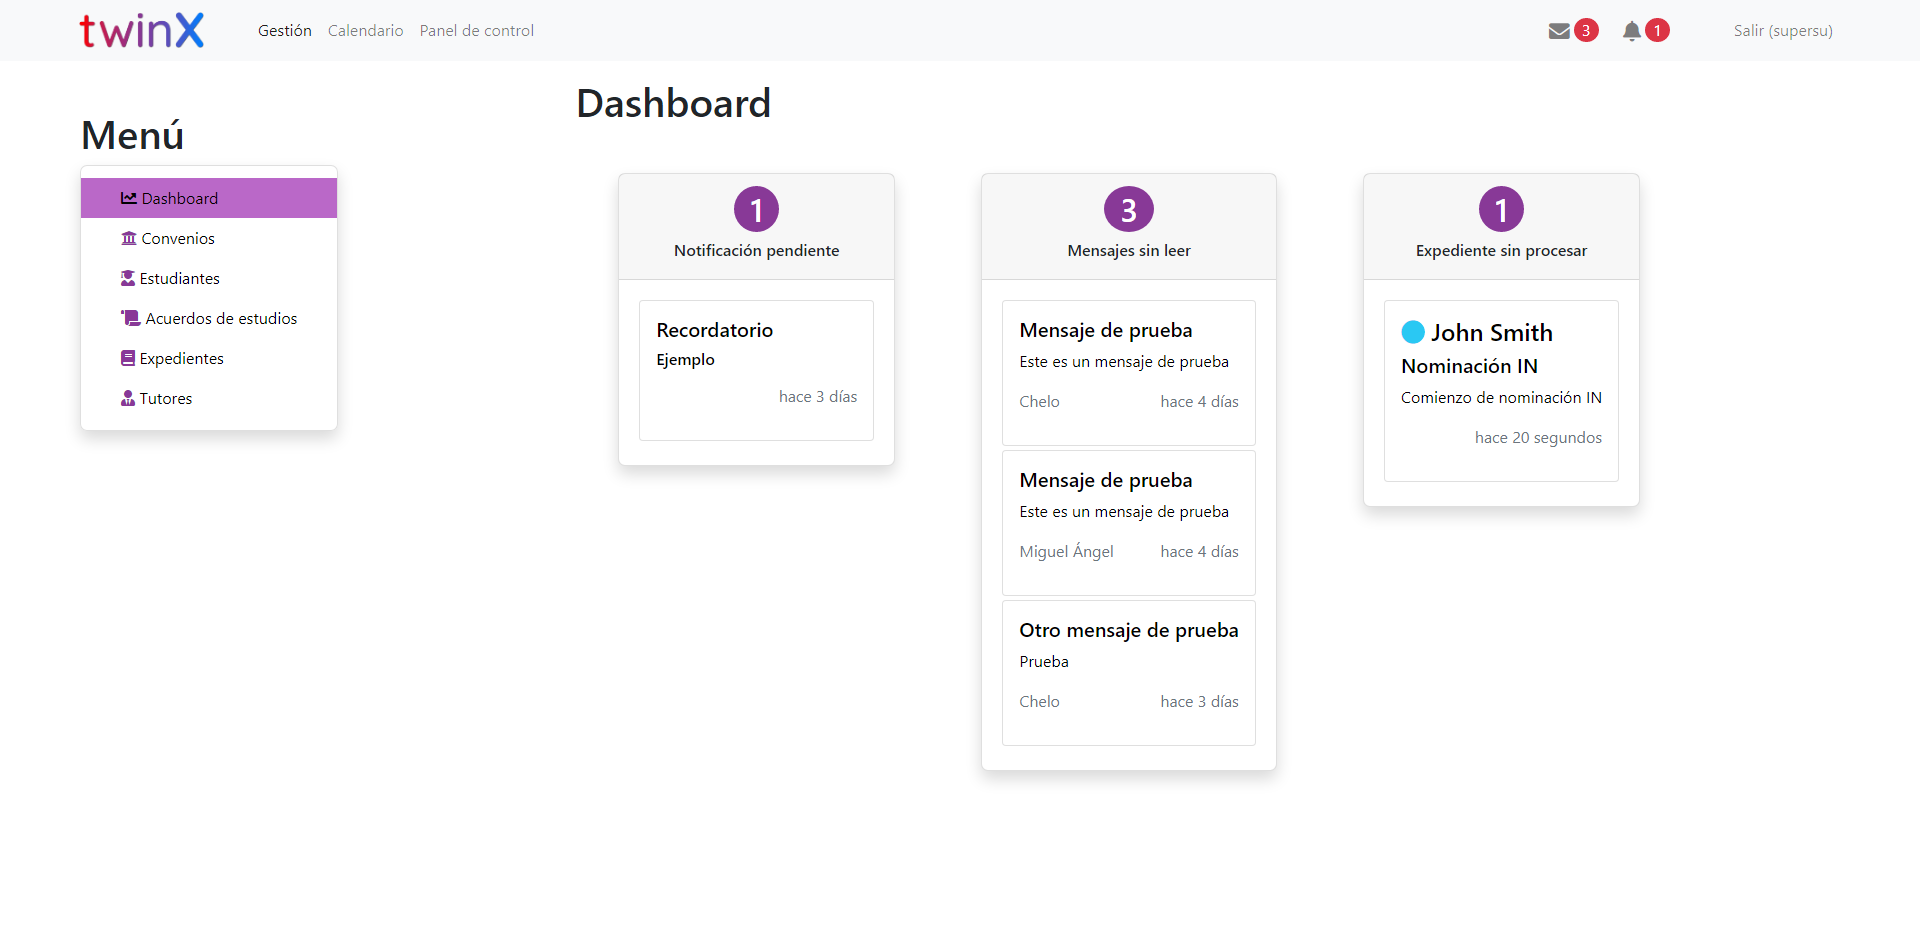
\includegraphics[width=\textwidth]{img/Wireframes/Gestión/dashboard.png}
	\caption[Wireframe de \textit{Dashboard}]{Wireframe del \textit{Dashboard} donde el usuario verá de un vistazo toda la información de mayor importancia al iniciar la aplicación}
	\label{fig:dashboardWF}
\end{figure}

\begin{figure}
	\centering
	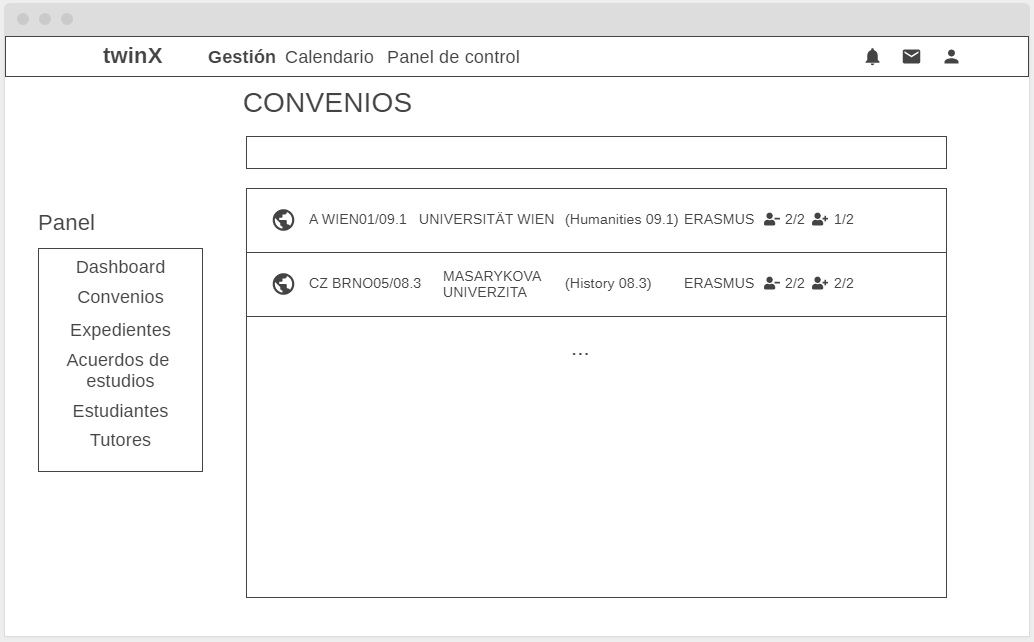
\includegraphics[width=\textwidth]{img/Wireframes/Gestión/convenios_lista.png}
	\caption{Wireframe de lista de convenios}
	\label{fig:convenios_listaWF}
\end{figure}

\begin{figure}
\centering
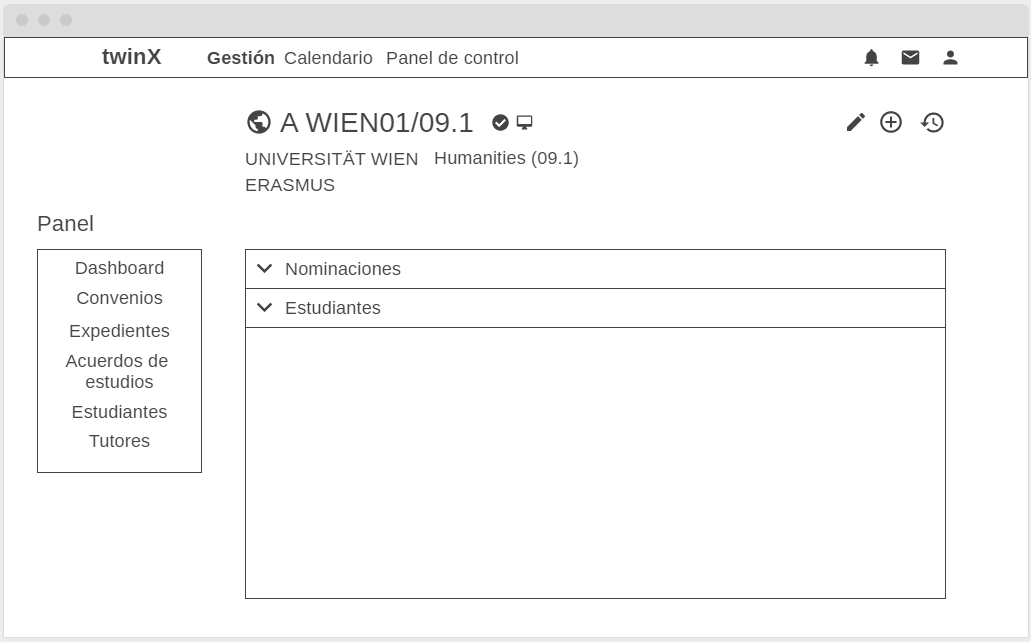
\includegraphics[width=\textwidth]{img/Wireframes/Gestión/vista_convenio_básica_contraída.png}
\caption[Wireframe de vista de convenio básica]{Wireframe de vista de convenio básica. Secciones contraídas.}
\label{fig:vista_conv_basica_contWF}
\end{figure}

\begin{figure}
	\centering
	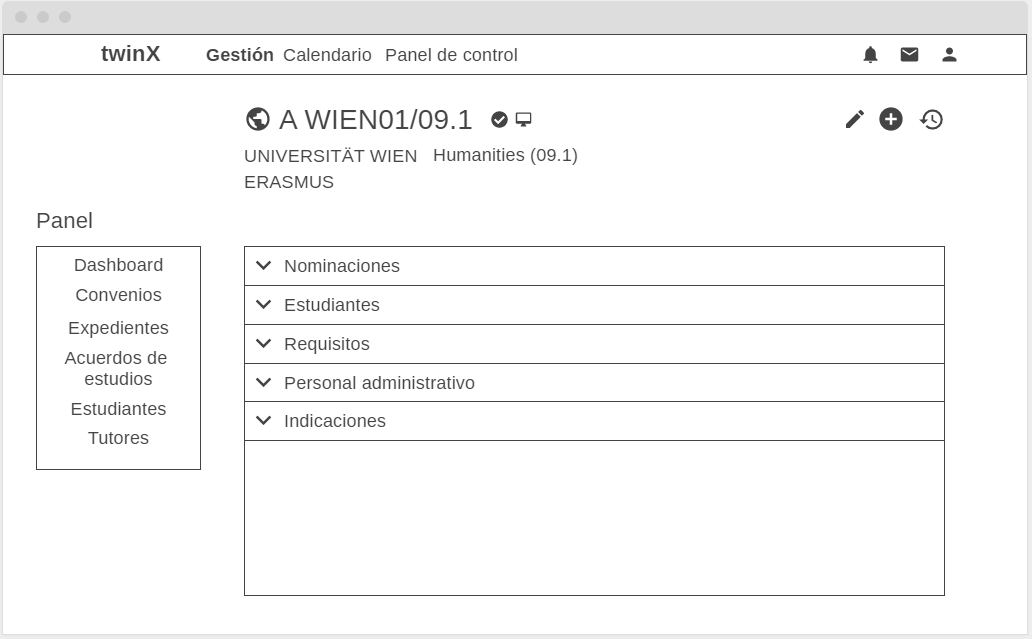
\includegraphics[width=\textwidth]{img/Wireframes/Gestión/vista_convenio_avanzada_contraída.png}
	\caption[Wireframe de vista de convenio avanzada]{Wireframe de vista de convenio avanzada. Secciones contraídas. Acceso desde el botón «+» de la botonera en la esquina superior derecha del contenido principal.}
	\label{fig:vista_conv_avanzada_contWF}
\end{figure}

\begin{figure}
	\centering
	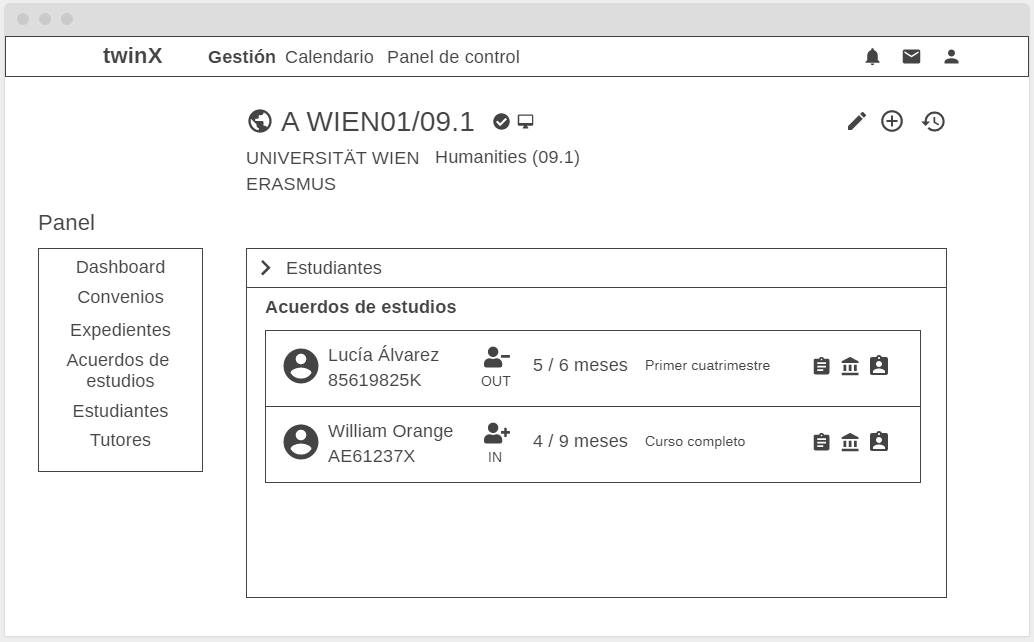
\includegraphics[width=\textwidth]{img/Wireframes/Gestión/vista_convenio_extendida.png}
	\caption[Wireframe de vista de convenio extendida]{Wireframe de vista de convenio extendida, donde se pueden ver los detalles de una o varias secciones en concreto bajo demanda.}
	\label{fig:vista_conv_extendidaWF}
\end{figure}

\begin{figure}
	\centering
	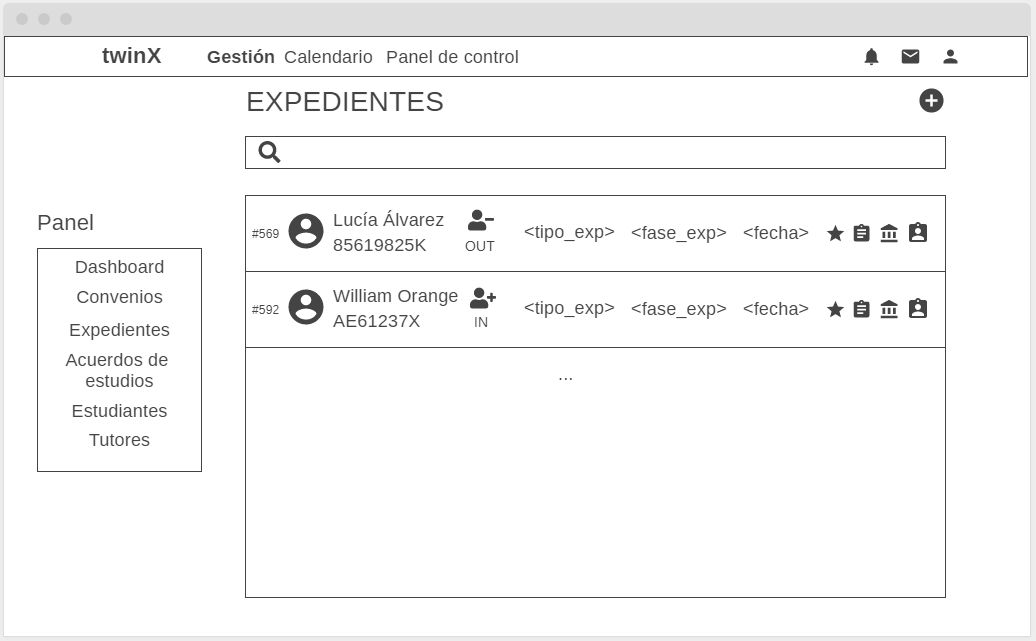
\includegraphics[width=\textwidth]{img/Wireframes/Gestión/expedientes_lista.png}
	\caption{Wireframe de lista de expedientes}
	\label{fig:expedientes_listaWF}
\end{figure}

\begin{figure}
	\centering
	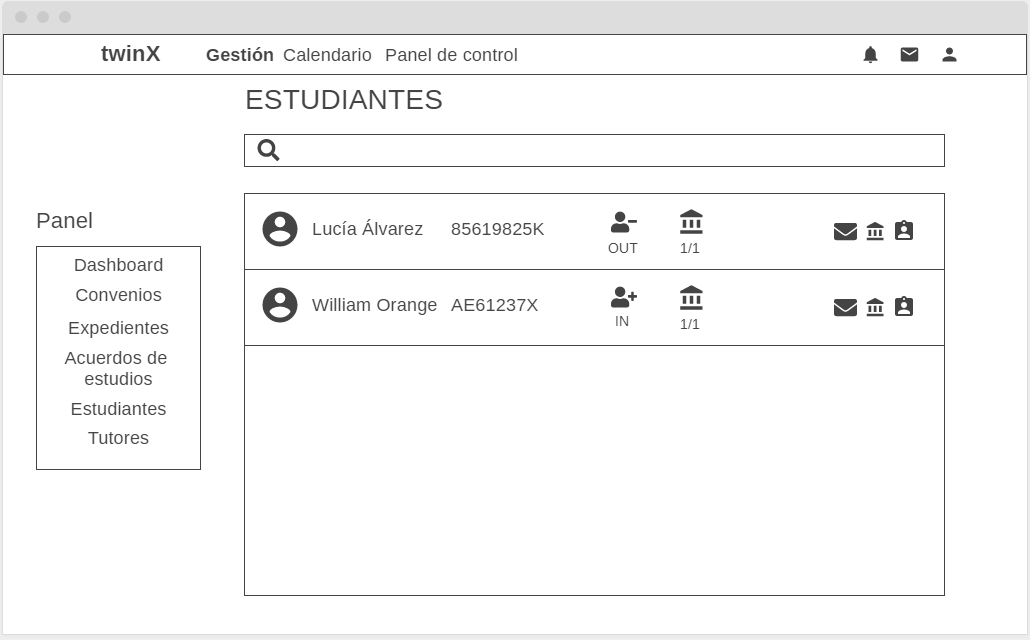
\includegraphics[width=\textwidth]{img/Wireframes/Gestión/estudiantes_lista.png}
	\caption{Wireframe de lista de estudiantes}
	\label{fig:estudiantes_listaWF}
\end{figure}

\begin{figure}
	\centering
	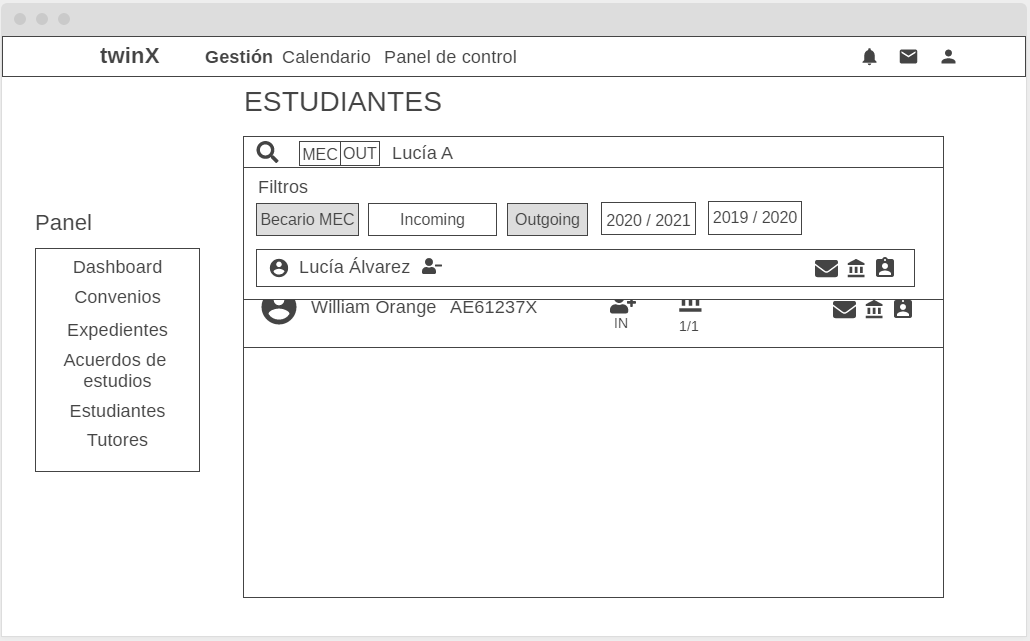
\includegraphics[width=\textwidth]{img/Wireframes/Gestión/búsqueda.png}
	\caption[Wireframe de búsqueda]{Wireframe de búsqueda. Diálogo modal, desplegable desde la barra. Capacidad de filtrado}
	\label{fig:busquedaWF}
\end{figure}

\begin{figure}
	\centering
	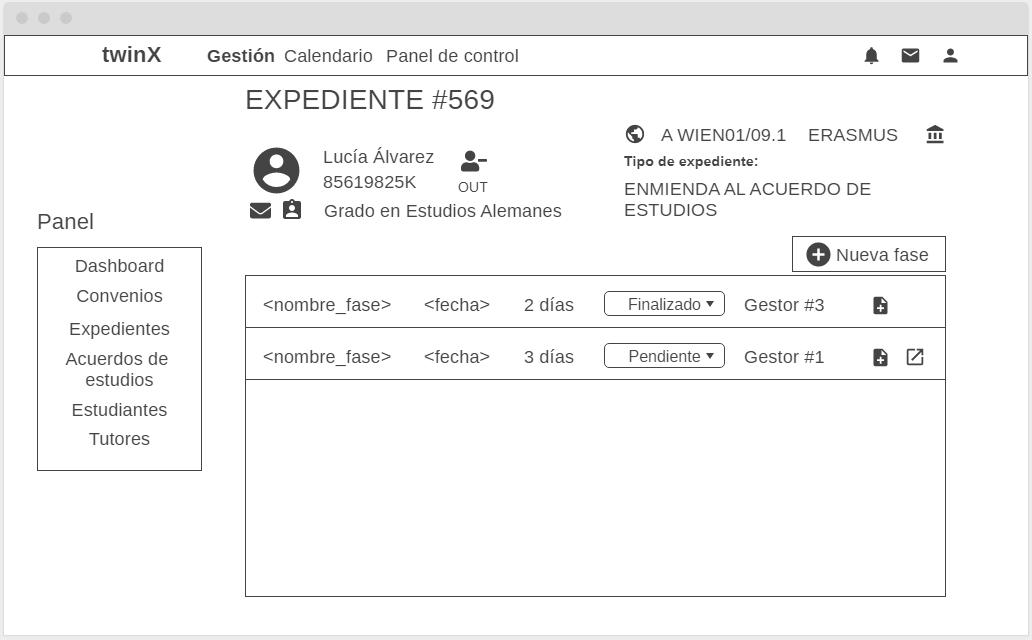
\includegraphics[width=\textwidth]{img/Wireframes/Gestión/expediente_detalle.png}
	\caption{Wireframe de detalle de expediente}
	\label{fig:expediente_detalleWF}
\end{figure}

\begin{figure}
	\centering
	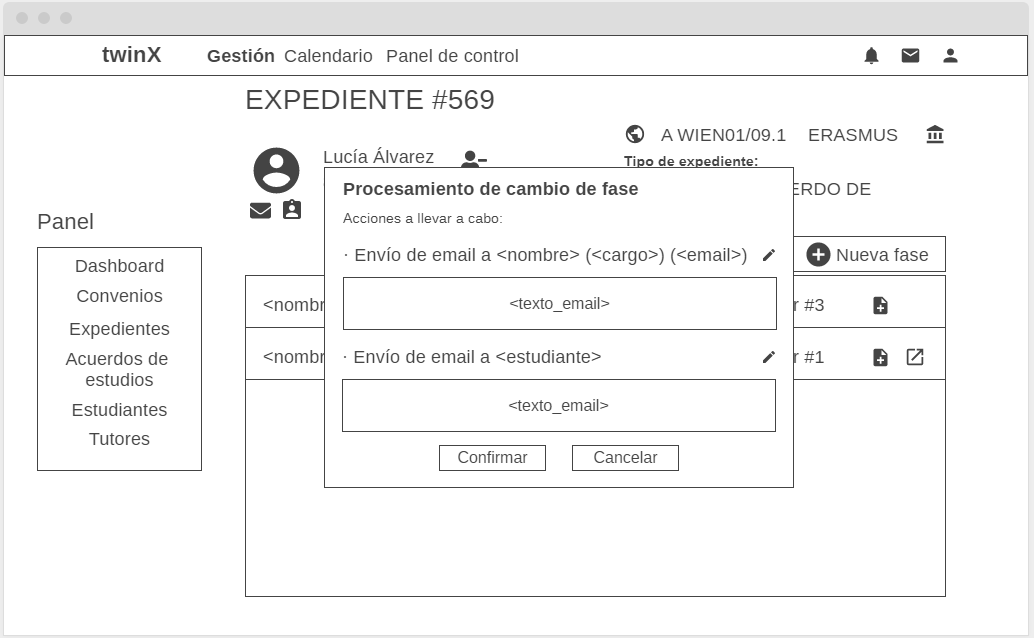
\includegraphics[width=\textwidth]{img/Wireframes/Gestión/cambio_fase.png}
	\caption[Wireframe del modal de cambio de fase]{Wireframe del modal de cambio de fase. Advierte sobre las acciones a llevar a cabo tras la tramitación del cambio de fase en un expediente concreto.}
	\label{fig:cambio_faseWF}
\end{figure}

\begin{figure}
	\centering
	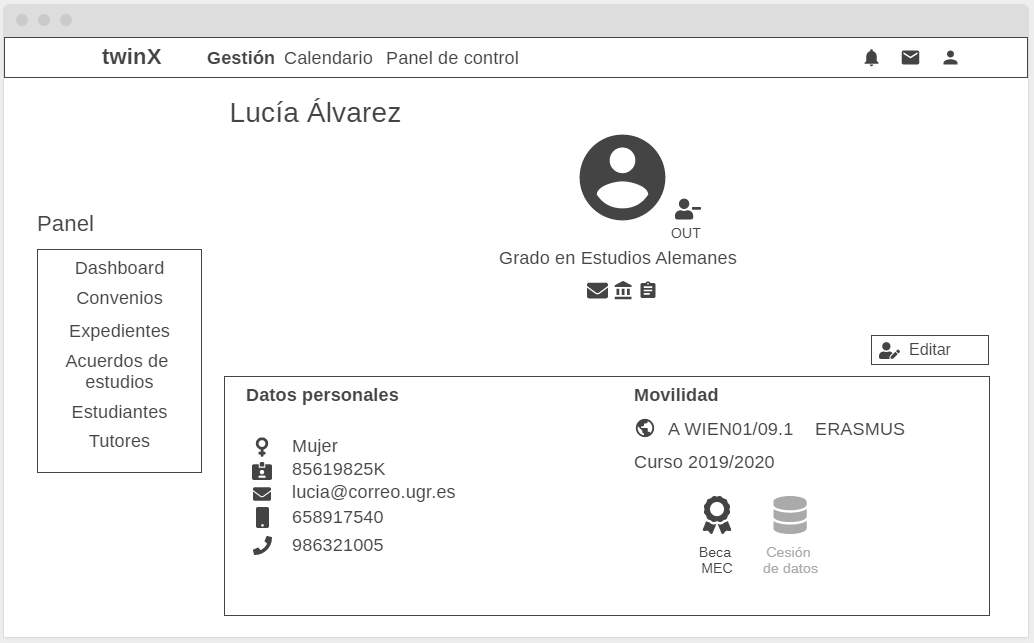
\includegraphics[width=\textwidth]{img/Wireframes/Gestión/estudiante_detalle.png}
	\caption{Wireframe de la vista de detalle de un estudiante}
	\label{fig:estudiante_detalleWF}
\end{figure}

%%PROVISIONAL PARA SEPARAR AMBOS CONJUNTOS DE WIREFRAMES
\newpage

\subsection{Wireframes del módulo de calendario}

Por su parte, los bocetos diseñados para el módulo del calendario son los siguientes:

\begin{itemize}
	\item \textbf{\hyperref[fig:eventos_listaWF]{Lista de eventos}:} alberga todos los eventos que se han creado en el sistema, con la información más relevante sobre los mismos y acceso a acciones como editar y eliminar.
	\item \textbf{\hyperref[fig:notificaciones_listaWF]{Lista de notificaciones}:} como los mensajes, recordatorios y/o avisos de tareas pendientes, que aparecerán en este menú, accesible también desde la barra persistente situada en la cabecera de la aplicación.
	\item \textbf{\hyperref[fig:nuevo_eventoWF]{Vista de creación de un evento}:} respeta en la medida de lo posible la vista de creación de un nuevo evento en TWINS, con los elementos esenciales. Si bien es cierto que podría no ser la más inmediata a la hora de pensar en una interfaz similar, se ha tratado de ajustar a las necesidades reales de los usuarios finales. En este caso, se pretende permitir la inclusión de un número indefinido de avisos para con el evento, lo cual es extensible al ámbito de las tareas asociadas al mismo evento (en TWINS se tenían siempre dos, lo que obligaba a ocupar más espacio en las tablas de la base de datos, sobre todo para aquellos eventos donde ni siquiera había un solo aviso definido).	
\end{itemize}

\begin{figure}
	\centering
	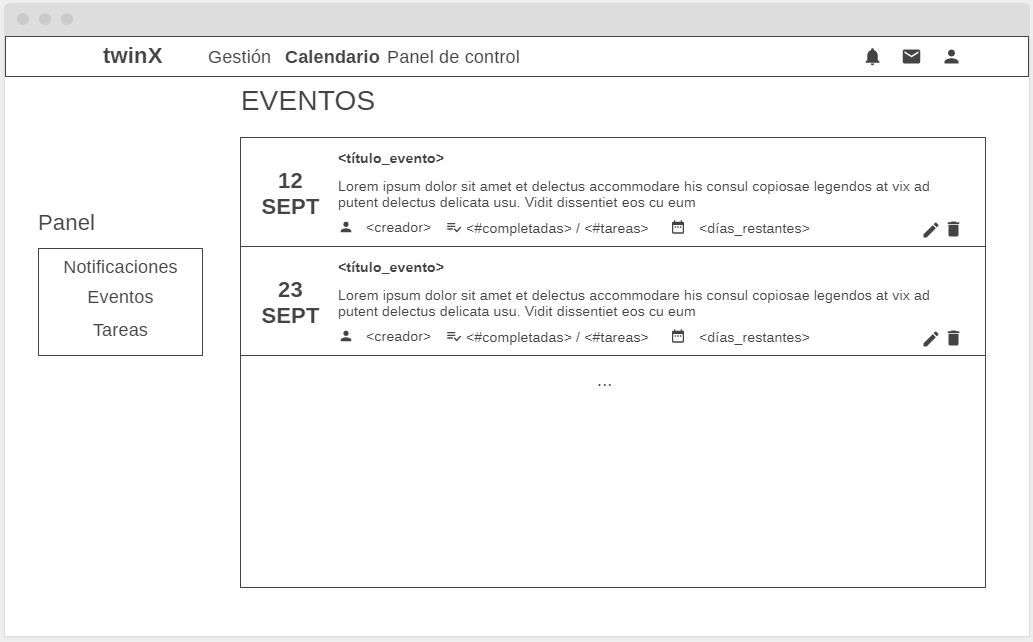
\includegraphics[width=\textwidth]{img/Wireframes/Calendario/eventos_lista.png}
	\caption{Wireframe de lista de eventos}
	\label{fig:eventos_listaWF}
\end{figure}

\begin{figure}
	\centering
	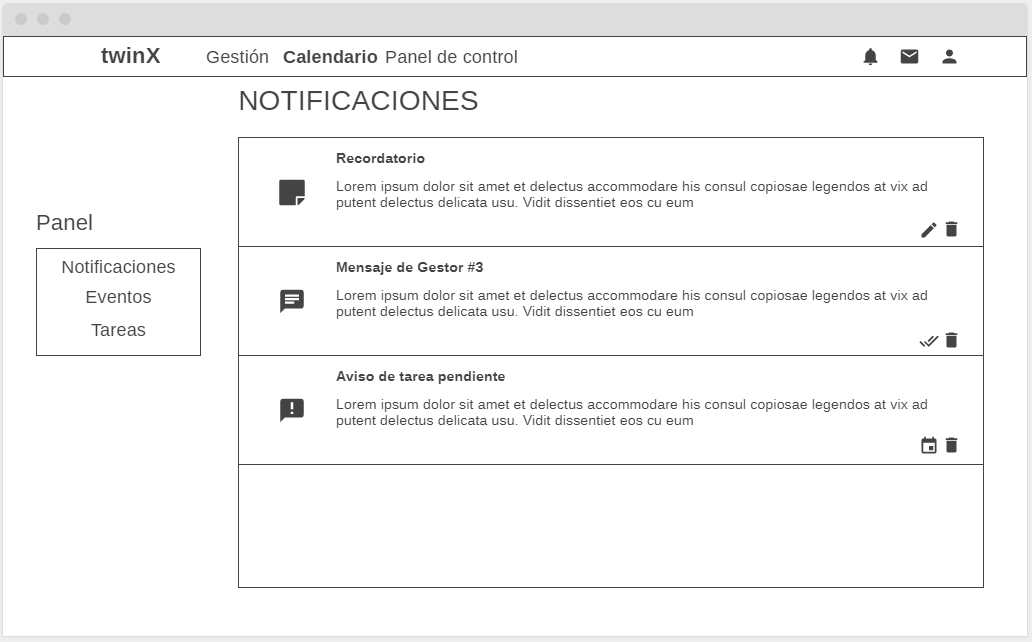
\includegraphics[width=\textwidth]{img/Wireframes/Calendario/notificaciones_lista.png}
	\caption[Wireframe de lista de notificaciones]{Wireframe de lista de notificaciones. Pueden aparecer tres tipos de notificaciones, dependiendo del tipo de mensaje recibido o generado por la propia plataforma (a través de avisos y/o recordatorios)}
	\label{fig:notificaciones_listaWF}
\end{figure}

\begin{figure}
	\centering
	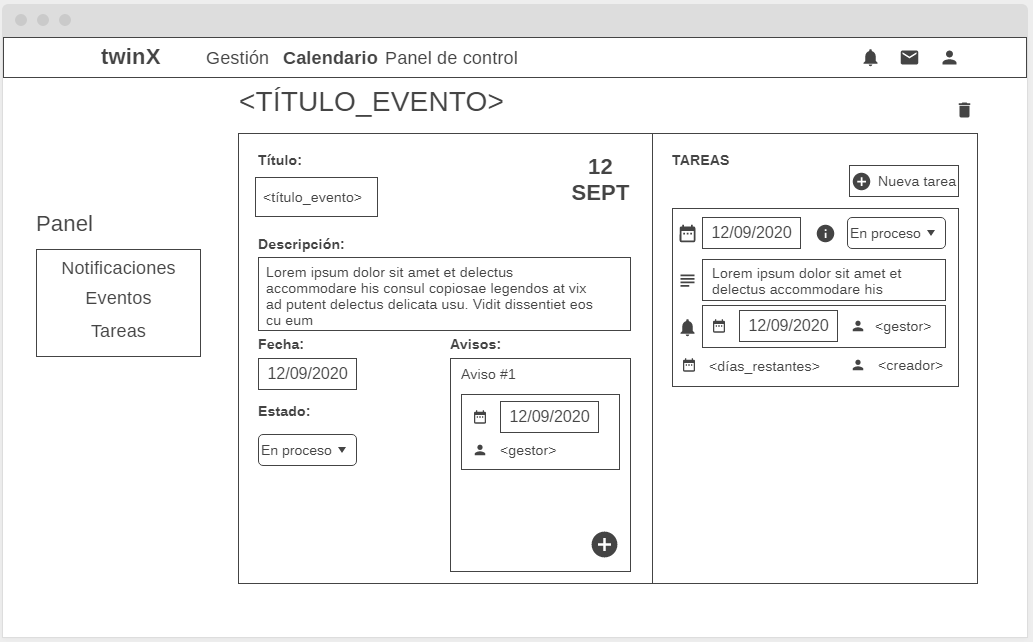
\includegraphics[width=\textwidth]{img/Wireframes/Calendario/nuevo_evento.png}
	\caption[Wireframe de creación de un evento]{Wireframe de creación de un evento. Se distinguen dos vistas: la información del evento en general (izquierda) y la de sus subtareas (derecha)}
	\label{fig:nuevo_eventoWF}
\end{figure}



